

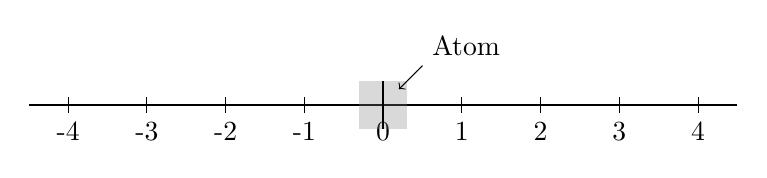
\begin{tikzpicture}
    % Draw the number line
    \draw[thick, -] (-4.5,0) -- (4.5,0);

    % Draw ticks and labels
    \foreach \x in {-4, -3, -2, -1, 0, 1, 2, 3, 4} {
        \draw (\x, 0.1) -- (\x, -0.1);  % tick marks
        \node[below] at (\x, -0.1) {\x}; % labels
    }

    % Draw shaded area around zero
    \fill[gray, opacity=0.3] (-0.3, -0.3) rectangle (0.3, 0.3);
    \draw[thick] (0, -0.3) -- (0, 0.3);  % thicker tick mark at zero

    % Draw label with arrow
    \draw[->] (0.5, 0.5) -- (0.2, 0.2);
    \node[above right] at (0.5, 0.5) {Atom};
\end{tikzpicture}

